\chapter{A Key-Value Store with Serializable Transactions for NVRAM}
\label{ch:concept}

The aim of this thesis is to design a \ac{KVS} with affordable serializable
transactions by exploiting the benefits of \ac{NVRAM}. In order to provide the
necessary groundwork, the previous chapters give an overview on recent research
in \ac{NVRAM}, \ac{KVS}, and concurrency control in databases. It is further
pointed out that, as of this writing, there appears to be no previous work on
leveraging \ac{NVRAM} for concurrency control in \acp{KVS} or \acp{MMDB},
respectively. While recent works primarily see \ac{NVRAM} as a means to reduce
recovery overhead, this thesis explores a different approach.

As mentioned in Chapter \ref{ch:kvs}, many transaction processing systems do not
support or encourage serializable transactions due to severe performance
degradation. Therefore, the idea is to use the benefits of \ac{NVRAM} to make
serializable transactions affordable. While this may not provide the highest
possible transaction throughput, the aim is to achieve performance on a par with
non-serializing solutions for traditional storage. In other words, instead of
increasing maximum performance, this work attempts to increase performance with
maximum consistency.

\ac{NVRAM} is especially significant for memory-resident databases as data no
longer needs to be copied to a much slower storage device for recoverability.
Also, restarts can be near-instantaneous as all data is already in memory and
does not need to be fetched. Therefore, the proposed concept is exclusively
targeted at \ac{MMDB}. Given the vast complexity of fully-featured in-memory
\ac{DBMS}, it seems appropriate, for an initial study, to resort to much more
manageable \ac{KVS}. Based on whether the approach turns out to work well for
\ac{KVS}, it may still be applied on \ac{MMDB} in future work.

This chapter presents the concept for an \ac{NVRAM}-aware \ac{KVS} with
serializable transactions. After a brief overview in the next section,
follow-up sections outline the architecture, concurrency control, and
consistency measures.

\section{Overview}
\label{ch:concept-overview}
This section provides an overview on the concept of this work. For this purpose,
goals, assumptions, and design constraints are outlined. The section concludes
with an outline of the desired \ac{API} and practical examples.

\subsubsection{Goal}

The intent of this thesis is to determine whether \ac{MMDB} could exploit
\ac{NVRAM} to make transactions with strong consistency affordable. Given the
overwhelming complexity of full-scale \ac{DBMS}, this work resorts to in-memory
\ac{KVS}. \ac{NVRAM} significantly reduces the required recovery overhead. While
others have used this circumstance to increase transaction throughput alone,
this work chooses to leverage the headroom to compensate for the cost of
serializability. The goal is to design a serializing in-memory \ac{KVS} for
\ac{NVRAM} which performs on par with non-serializing \ac{KVS} based on volatile
\ac{RAM}.

\subsubsection{Assumptions}

The concept is based on several assumptions concerning both technical aspects
and workloads characteristics.

\paragraph{Hardware}

In order to take advantage of concurrency, the concept is designed for
multi-core architectures. While this increases the number of threads that can be
run in parallel, it also introduces synchronization issues for access to shared
memory which must be handled with care. However, to keep complexity manageable,
the concept refrains from distributed computing and targets single-node
databases. In accordance with recent research, it is assumed that volatile
\ac{RAM} will continue to be present and share the same memory interface with
\ac{NVRAM}. This reduces individual bandwidths but enables uniform access
methods. It is further assumed that target systems provide sufficient hardware
and software facilities to manage \ac{NVRAM}. Details concerning crash
consistency are provided in Chapter \ref{ch:concept-consistency}

\paragraph{Workloads}

When designing systems and transaction processors, in particular, it is helpful
to know in advance which kind of workloads are expected or should be given
priority. Given that many \ac{MMDB} are dominated by read operations
\cite{andrei2017sap}, this work is intended for read-mostly workloads. While
read-only transactions are supported, there seems to be no hard evidence on the
importance or quantity of such transactions. Likewise, long-running transactions
are not handled separately, as their share could not be determined.

\subsubsection{Design Constraints}

\paragraph{In-Memory Operation}

Since the intent of this work is to evaluate opportunities of \ac{NVRAM} for
\ac{MMDB}, the target \ac{KVS} must hold all its data in volatile or
non-volatile main memory with no disk storage involved. This way, access
latencies are limited to main memory rather than slower disk storage or
\ac{SSD}.

\paragraph{Transactions}

Contrary to full-grown \ac{MMDB}, a number of \ac{KVS} does not support
transactions that span multiple primitive operations. However, in order to allow
conceptual conclusions to \ac{MMDB}, it is important to maintain sufficient
generality. Therefore, the concept requires full-featured transactions as in
\ac{MMDB}. As a result, multiple operations, such as reading or writing an item,
may be enclosed within a transaction. Likewise, full ACID support is required to
guarantee sound transactional semantics. In order to guarantee strong
consistency and isolation in the presence of concurrent transactions,
serializability is a central requirement. Note that, in contrast to some
\ac{KVS} which are designed as caches the target \ac{KVS} in this work supports
durability. Concerning the nature of key-value pairs, this work imposes no
restrictions on their datatypes. Still, implementations are free to limit the
length of keys, for instance, if the underlying data structure requires it.

\subsubsection{API}

Given the simplistic nature of \ac{KVS}, this concept anticipates a narrow
\ac{API} that features the very basic building blocks of transactional
semantics. The \ac{API} can be described as a tuple of three instruction sets.
First, there are routines to create or manage instances of the \ac{KVS}. The
second set consists of routines to start and end transactions. Transactions are
managed through handles which are retrieved when creating them. Such transaction
handles are required for the third set of instructions, namely inserting or
deleting pairs and retrieving values. Table \ref{tab:api} gives an outline of
the intended \ac{API}.

\begin{figure}[!h]
    \centering
    \begin{tabular}{|l|l|}
        \hline
        \textbf{Function}          & \textbf{Description} \\
        \hline
        kvstore()                  & Create a key-value store instance \\
        begin() : tx               & Start a transaction \\
        begin\_ro() : tx            & Start a read-only transaction \\
        commit(tx) : bool          & Commit a transaction \\
        abort(tx) : void           & Abort a transaction \\
        get(key, tx) : value       & Retrieve value for a given key \\
        put(key, value, tx) : void & Insert a key-value pair \\
        remove(key, tx) : void     & Remove a key-value pair \\
        \hline
    \end{tabular}
    \caption{API of the intended key-value store.}
    \label{tab:api}
\end{figure}

This \ac{API} is sufficient to power a basic database with transactional
semantics. Listing \ref{lst:api_ex} shows an example where a transaction checks
whether the balance is negative and, if so, applies a penalty.

\begin{lstlisting}
kvstore kvs;

/* ... lots of transactions ... */

auto tx = kvs.begin();
auto deb = kvs.get("debit", tx);
auto sav = kvs.get("saving", tx);
if (getBalance(sav, deb) < 0.0) {
	kvs.put("debit", applyInterest(deb), tx);
}
tx->commit();
\end{lstlisting}\label{lst:api_ex}

For an example with concurrent transactions, see Listing \ref{lst:api_ex2}.
Here, two transactions are executed concurrently which leads to a data race.

\todo[inline]{Insert listing/control flow for concurrent transactions}


\section{System Architecture}
\label{ch:concept-system}
The \ac{KVS} is designed for multi-core architectures and relies on both
volatile and non-volatile memory attached to the system memory interface. In
order to take advantage of both types of memory, the \ac{KVS} is designed as a
two-level store which only updates \ac{NVRAM} when a transaction commits.
Consistency across crashes is ensured with existing hardware primitives and
upcoming platform features. Concurrent transactions are controlled by a
serializable variant of \ac{SI}. Background on these design decisions is given
below.

Designing a runtime-critical software such as databases not only involves
knowledge about expected workloads but also about the underlying computing
device. While workloads have been discussed earlier, this section describes the
system architecture of the intended \ac{KVS}.

\subsubsection{Concurrency}

The \ac{KVS} is designed for a single-node architecture. Even though distributed
databases are fairly common, there seems to be no apparent reason for them to
reveal any more insight on leveraging \ac{NVRAM} for concurrency. Also,
distributed systems involve much more complex mechanisms such as consensus among
distributed transactions, all of which are beyond the scope of this work.
However, future work should investigate whether the conclusions of this work
also hold for distributed databases.

In order to achieve scalable transaction throughput through concurrency, the
target system is a multi-core architecture. That means, the system features one
or more processors with multiple cores, where each core may support multiple
hardware threads. On such a system, each transaction is executed in the context
of a thread which is scheduled and assigned to a processor core by the operating
system. Processors usually coordinate their work by communicating via some form
of chip interconnect. In order to preserve generality, this work makes no
assumptions concerning the nature of such interconnect networks.

\begin{figure}[h!]
    \centering
    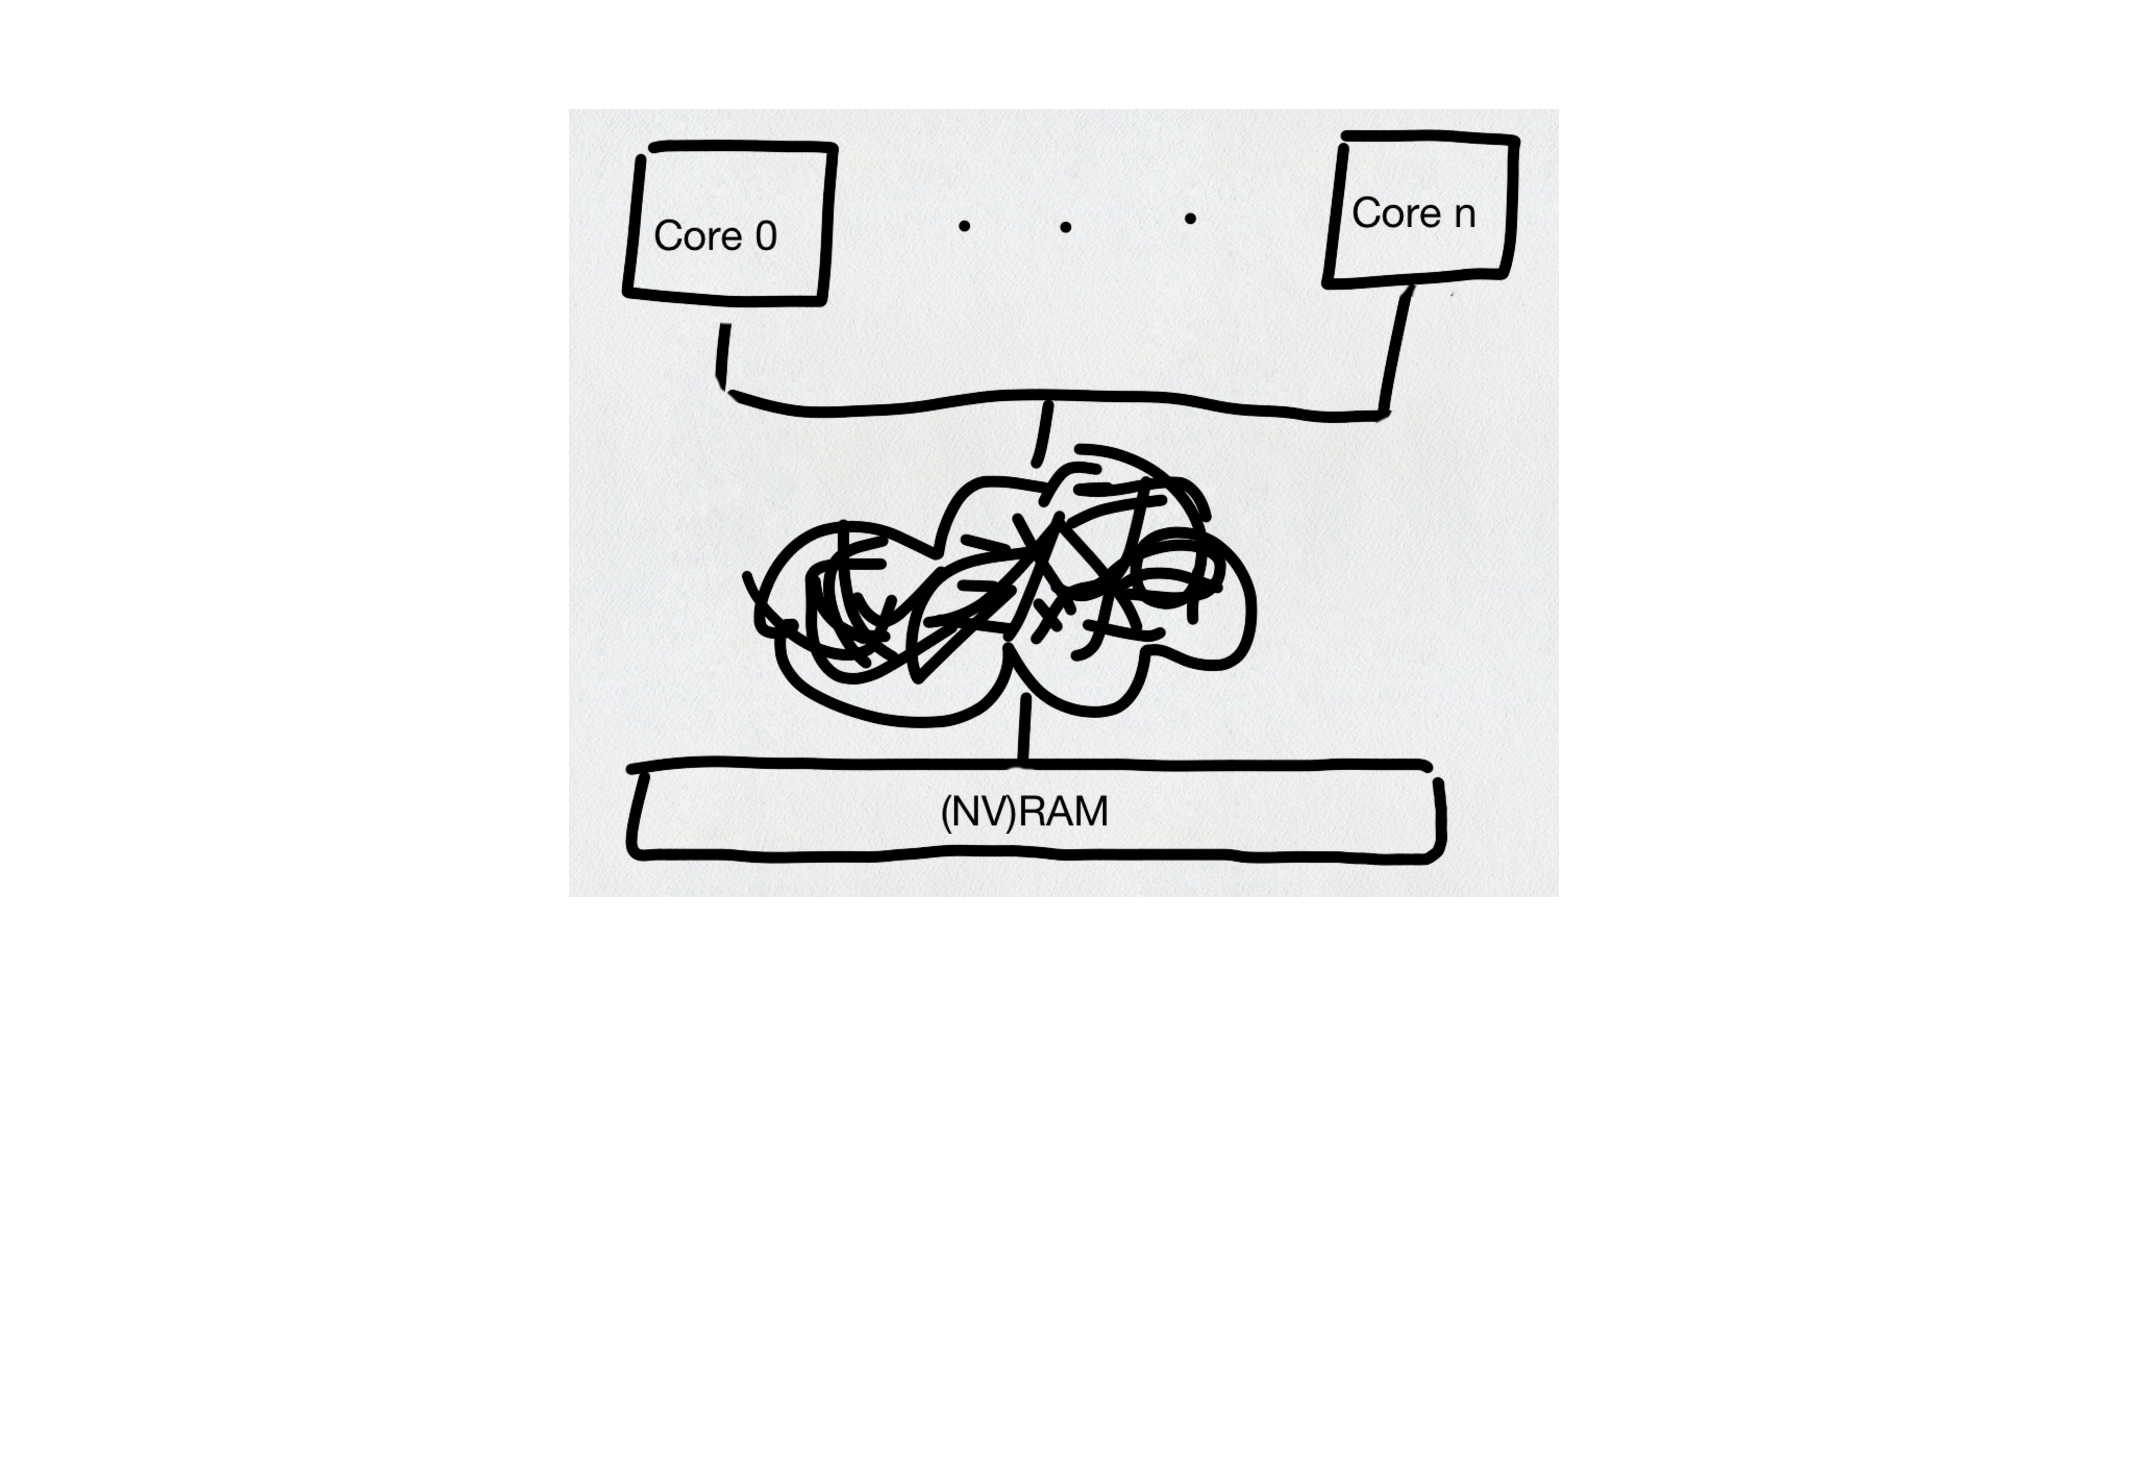
\includegraphics[scale=0.5]{figures/drafts/concept-sys-cpu.pdf}
    \caption{}
    \label{fig:concept-sys-cpu}
\end{figure}

\subsubsection{Memory Architecture}

Recent research shows that on traditional hardware it is advisable to continue
integrating volatile \ac{RAM} together with \ac{NVRAM}. The reason is that not
all data is meant to be durable which is especially true for \ac{NVRAM} where
crash consistency is linked with considerable overhead. Manufacturing \ac{NVRAM}
is still challenging, especially in terms of access latency and endurance, but
it is expected that these issues will be resolved in the near future. Therefore,
in an effort to combine the benefits of both technologies, the memory subsystem
is required to feature both volatile \ac{RAM} and \ac{NVRAM}. In accordance with
recent research it is assumed that both kinds of memory can be accessed through
the same memory interface. This work assumes a shared memory architecture. That
is, processors may have one or more private cache levels but main memory is
accessible to all processors. Conceptually, cache coherence is not required but
has the advantage that less effort is spent on coordinating concurrent access to
shared data.

The \ac{KVS} is designed to exclusively reside in main memory. All data that is
not required across restarts is stored in volatile \ac{RAM}, whereas all other
data are stored in \ac{NVRAM}. Multiple recent works have demonstrated that
\ac{NVRAM} can be used to build \ac{MMDB} without conventional non-volatile
storage such as hard drives. As a result, ensuring recovery, which has always
been an inherent bottleneck of \ac{MMDB}, can be eliminated. In addition,
near-instantaneous restarts become feasible. As a consequence, conventional
storage is not part of the concept for this \ac{KVS}. While such components may
very well be present in a system, they are never used to store any data of the
\ac{KVS} other than its binaries. This way, data access incurs no I/O and
restarts do not have to fetch data from slower storage devices. In return,
candidate systems must provide sufficient \ac{NVRAM} capacity to hold the entire
database.

\begin{figure}[h!]
    \centering
    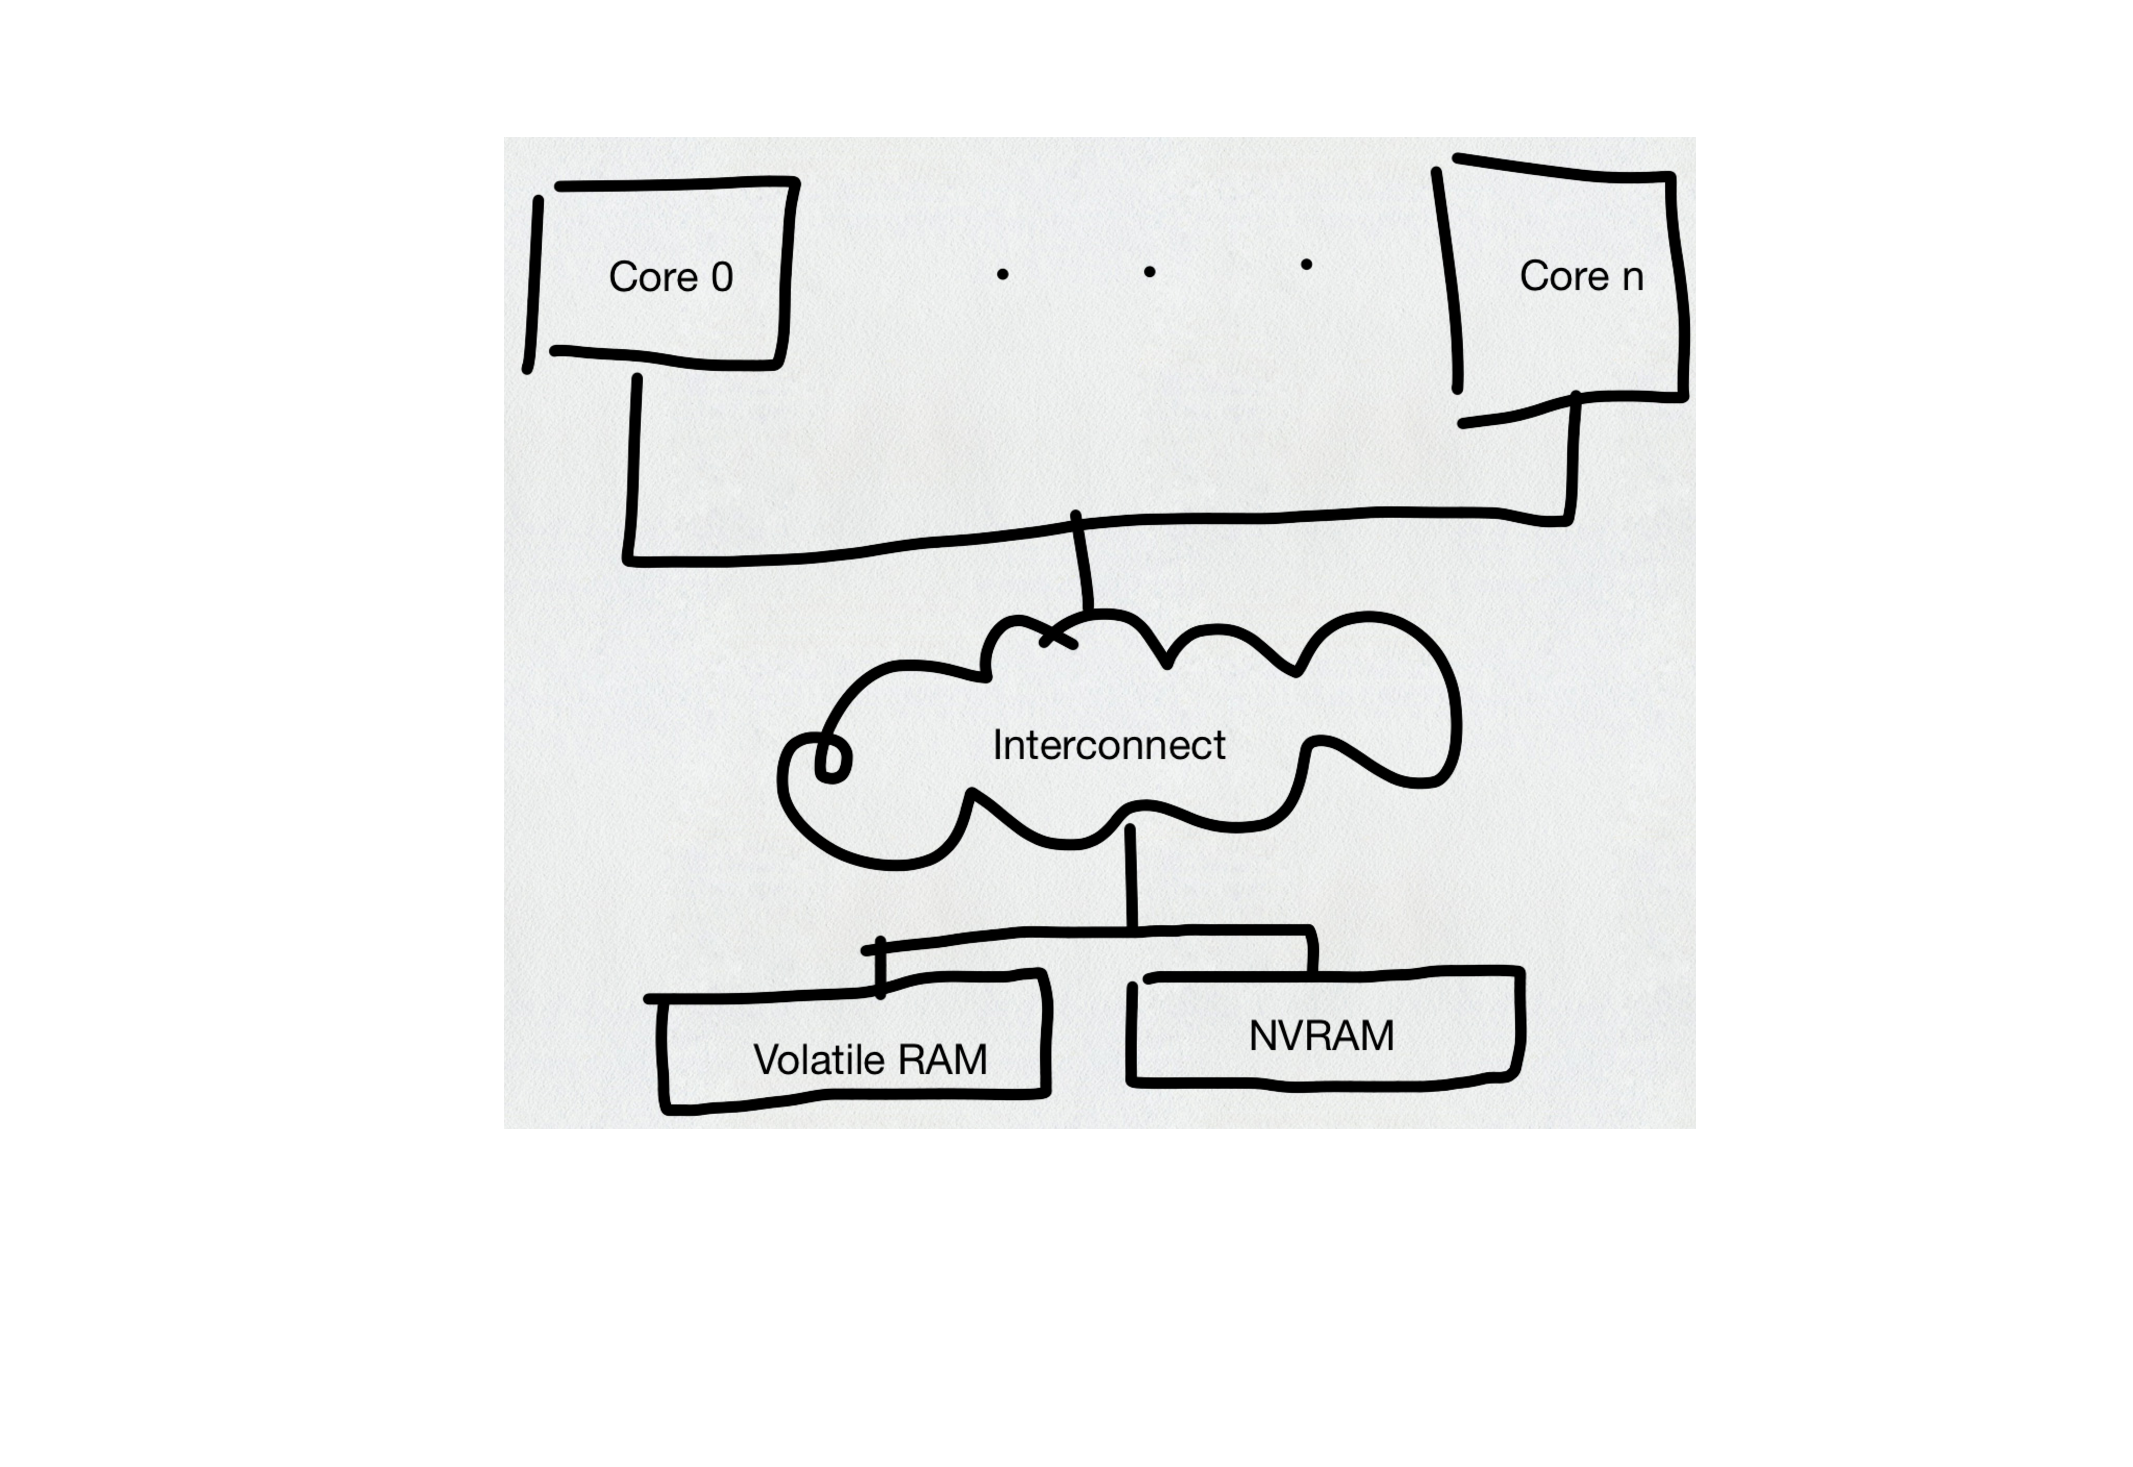
\includegraphics[scale=0.5]{figures/drafts/concept-sys-mem.pdf}
    \caption{}
    \label{fig:concept-sys-mem}
\end{figure}

A disadvantage of this approach is that the size of the database is bounded by
the amount of available \ac{NVRAM}. In contrast, \acp{MMDB} usually allow for
larger data sets by keeping frequently used data in memory, while others are
moved to slower mass storage media. However, main memory capacities have been
steadily growing and \ac{NVRAM} capacities are projected to have at least twice
the capacity of \ac{DRAM}. Another drawback is recoverability in case of device
failures. Mass storage not only scales better in terms of capacity, but it also
supports redundancy through \ac{RAID}, for instance. With \ac{NVRAM}, both
capacity and scalability are lower, so employing information redundancy may be
prohibitively expensive. Without such measures of fault tolerance, however, a
single failed \ac{NVRAM} module may lead to permanent data loss. This issue is
not within the scope of this thesis.


\section{Key-Value Store Design}
\label{ch:concept-kvs}
This section describes the software architecture of the \ac{KVS}. That includes
the operation principle in terms of transactions, storage, and concurrency as
well as the general structure.

\subsection{Two-Level Store}

As mentioned above, the \ac{KVS} resides entirely in main memory. This enables
fast access to all data within the database and makes swapping obsolete. In
return, the size of the database is bounded by the total \ac{NVRAM} capacity.
Apart from capacity, operating \ac{NVRAM} currently exhibits greater access
latencies compared to \ac{DRAM}. As pointed out in Chapter \ref{ch:nvram}, these
latencies mainly affect writes and are attributed to both technology parameters
and crash consistency measures. This work assumes, that even as technology
improves, crash consistency will continue to come a cost.

In an effort to mitigate these issues, the \ac{KVS} is designed to use volatile
\ac{RAM} in addition to \ac{NVRAM}. In order to achieve maximum performance, it
attempts to exploit the benefits of either technology while limiting the impact
of their drawbacks. For that purpose, the \ac{KVS} employs a two-level store
architecture as in \cite{bailey2013exploring}.

In a two-level store architecture, in-flight data from memory accesses may be
buffered in an intermediary storage medium. In this case, write operations are
buffered in volatile memory until their associated transaction commits. Only
when a transaction commits, all its updates are propagated to \ac{NVRAM}.
Otherwise, no user data is written to \ac{NVRAM}. Read operations are not
directly affected by the two-level store paradigm. In some cases, however, an
implementation may choose to buffer read operations, for instance to determine
serialization order.

The aim of the two-level store architecture is to reduce the impact of
\ac{NVRAM}-related latencies. Buffering updates to \ac{NVRAM} in volatile memory
has several advantages. First, updates are only posted to \ac{NVRAM} when they
need to be which can save both latency and memory bandwidth, especially when
aborts are frequent. Second, limiting updates to \ac{NVRAM} to commit phases
allows for bulk writes. This way, expensive consistency procedures do not have
to be performed repeatedly for a single transaction. Third, updated items in
volatile memory can be accessed with lower latencies, which is true for both
read and write operations. In the end, buffering updates also aids recovery, as
uncommitted data is guaranteed to be lost after a restart.

\begin{figure}[h!]
    \centering
    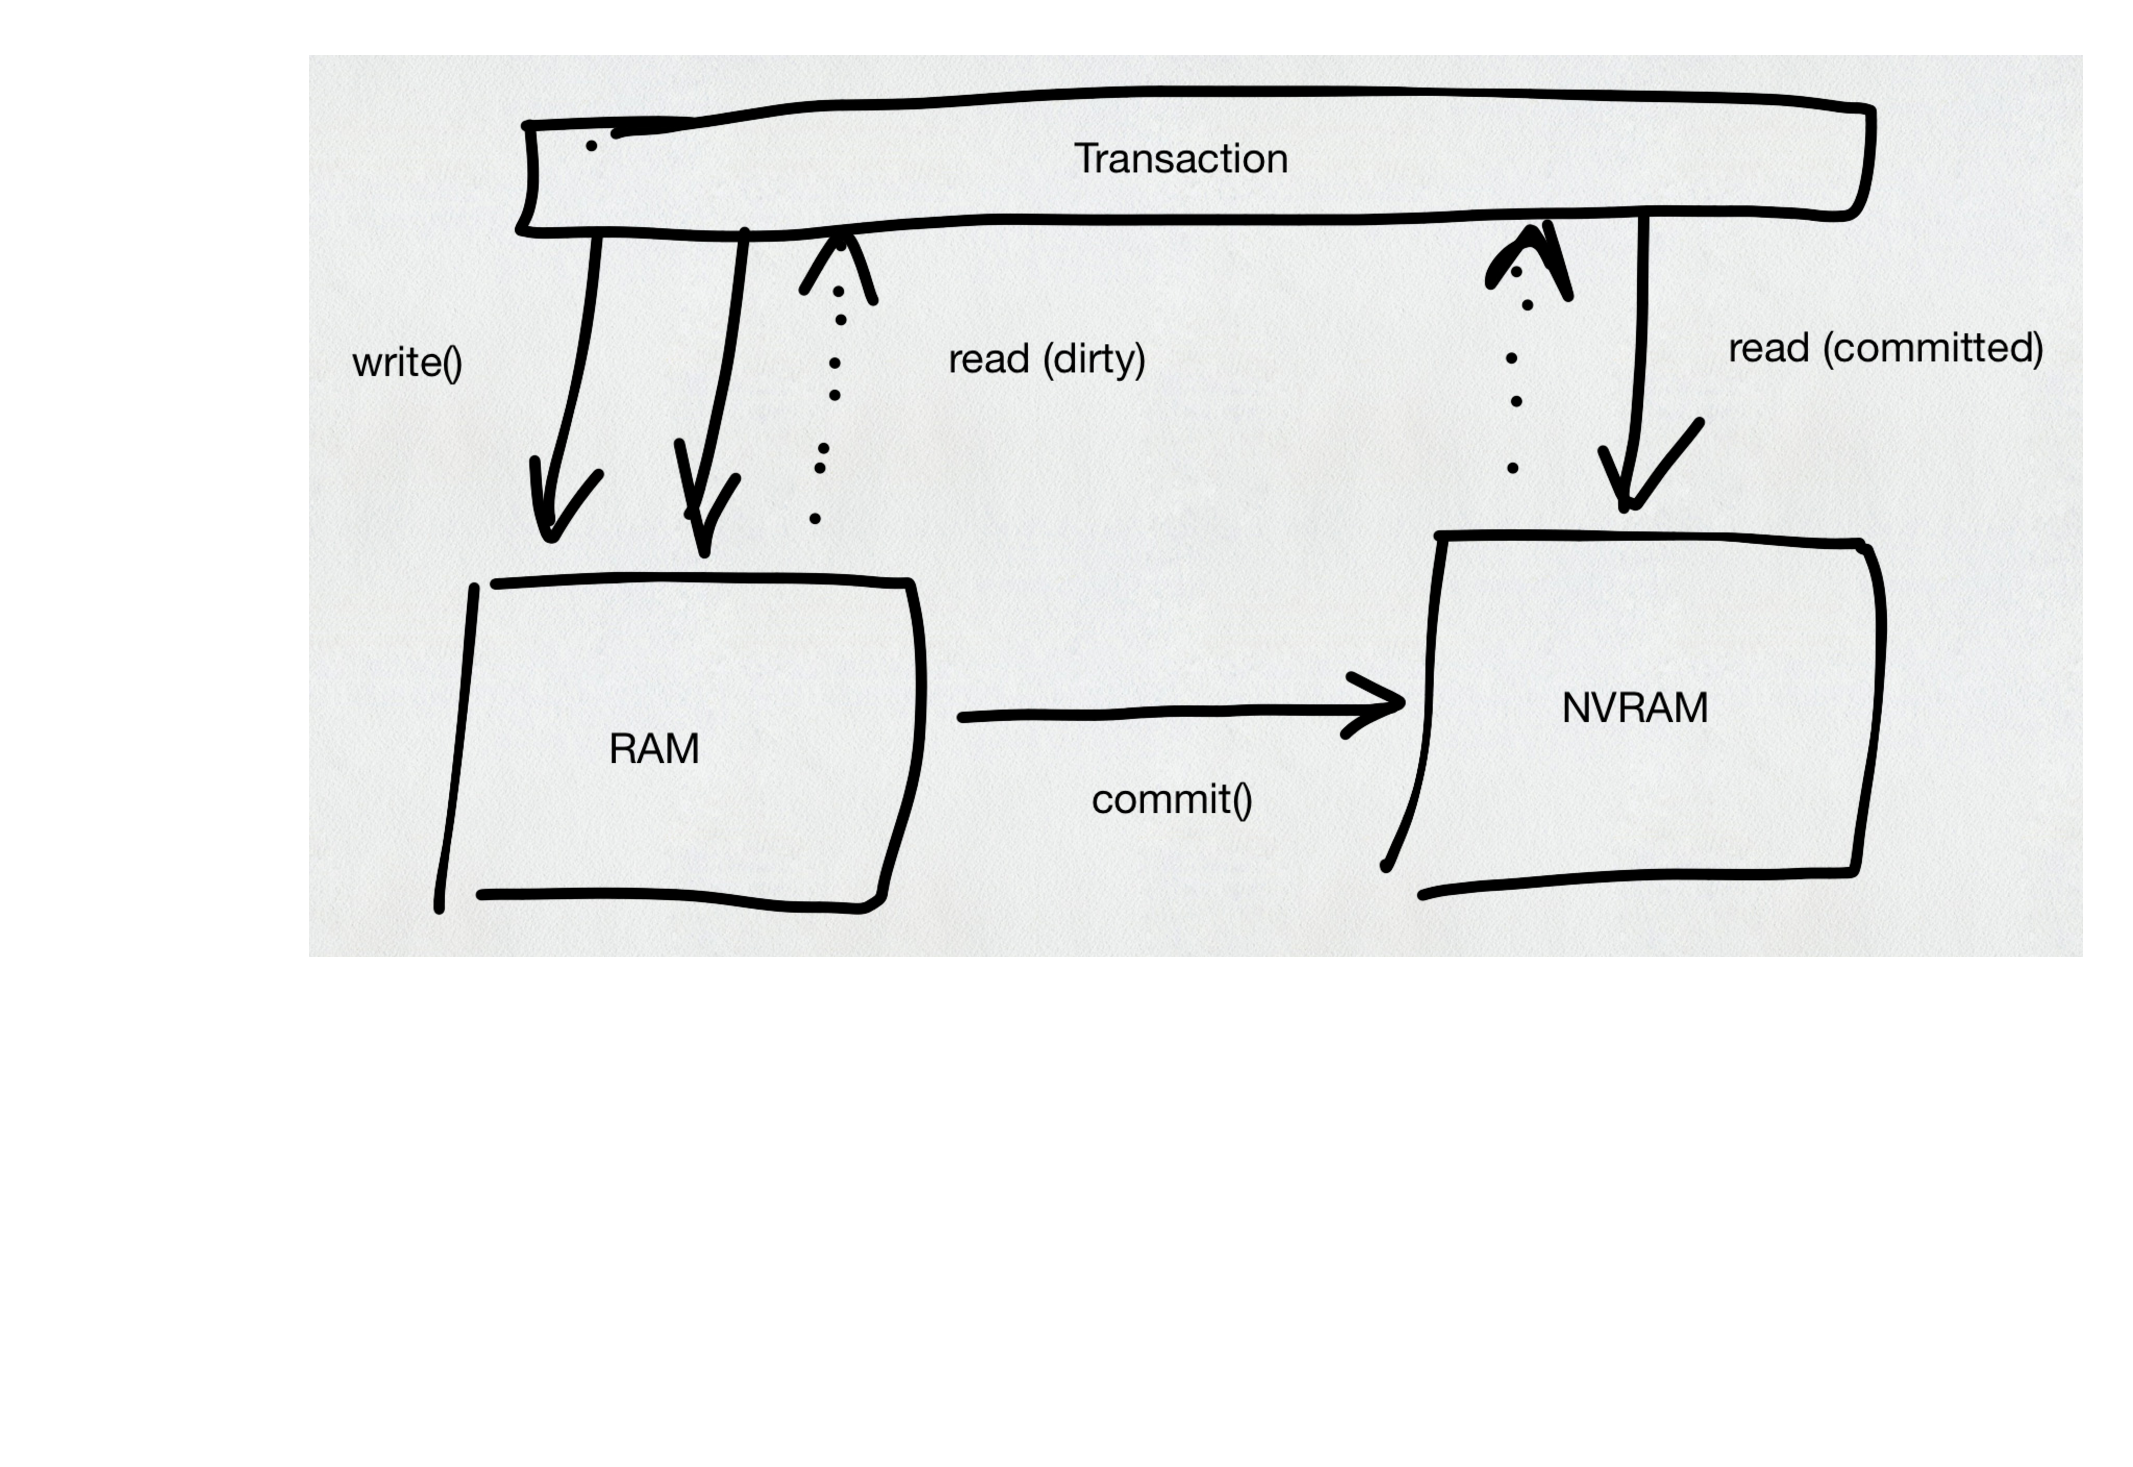
\includegraphics[width=\textwidth]{figures/drafts/concept-sys-two-level-store.pdf}
    \caption{}
    \label{fig:concept-two-level-store}
\end{figure}

\todo[inline]{phasen einer transaktion? genauer ablauf}

\subsection{Transactions}
\label{ch:concept-kvs-tx}

The \ac{KVS} supports full-featured and ACID-compliant transactions. Unlike
other works, this \ac{KVS} allows multiple operations to be enclosed in a single
transaction. The primary motivation behind this decision is to preserve
generality with regard to more complex \ac{DBMS}. Likewise, all transactions
must conform to the ACID properties to ensure data consistency. Nesting
transactions is not supported as use cases are too few to justify the additional
complexity.

Providing ACID support requires a conjunction of preventing erroneous behavior
and restoring a previously sane state if an error occurs.

\paragraph{Isolation}

The cornerstone of this work is to ensure isolation between concurrent
transactions, that is concurrent transactions cannot observe each others
uncommitted actions. This is achieved with the two-level store architecture and
a serializing \ac{MVCC} protocol.

Each transaction is run in a separate thread. All modifications within a
transaction are buffered in thread-local volatile memory as opposed to updating
in-place. As a result, the database in \ac{NVRAM} does not reflect uncommitted
changes and can therefore not be used to observe such activity. Technically,
threads could spy on each others change buffers but such behavior is neither
required nor intended.

Protecting transactions from observing concurrent updates, however, does not
imply transactionally consistent data. For this purpose, the \ac{KVS} employs a
serializing \ac{MVCC} protocol. When compared to locking-based approaches,
\ac{MVCC} protocols have shown better performance in read-intensive environments
and are used in many databases. In this case, the concrete protocol is a
serializing variant of \ac{SI} and serves two purposes: recovery and ensuring
all transactions behave as if run serially. On the one hand, timestamped
versions are used to keep track of modifications. On the other hand, a
copy-on-write mechanism is used to enable recoverable version histories without
logging. In order to achieve serializability, all read operations are tracked in addition to the usual change sets. On commit, a validation phase ensures that no read versions have been modified by other transactions. If validation fails, so does the corresponding transaction. For write-write conflicts, the first-updater-wins strategy is applied. This helps aborting conflicting transactions earlier than at commit which saves computing resources.

\paragraph{Atomicity}

Atomicity means that a transaction either succeeds as a whole or it fails
entirely. This means that any traces of a failed transaction must be either
neutral or reverted. As with isolation, atomicity is achieved by the two-level
store architecture and the concurrency control protocol. The former ensures that
only modifications of committing transactions are written to durable memory.
That way, an incomplete or failed transaction cannot be globally observed. In
addition, the \ac{SI} protocol allows the system to always retrieve the latest
committed version of an item. Even if an update to \ac{NVRAM} fails, the
\ac{KVS} can always go back to the latest committed version without performing
an actual rollback. However, in the event an update propagation to \ac{NVRAM} is
interrupted, partial write-backs may become durable. A typical scenario would be
a system crash or a power failure. In this case, the \ac{KVS} must ensure that
torn writes do not harm the consistency of data. Possible solutions for this
problem are recovery routines that locate and invalidate corrupted data or
designated bit fields that are guaranteed to be set only after the entire payload
has been written. The concrete recovery method to be used is
implementation-defined. For details, see Chapter \ref{ch:impl}.

\paragraph{Durability \& Consistency}

Ensuring durability and consistency with \ac{NVRAM} requires special attention
and is covered in Chapter \ref{ch:concept-consistency}.

\subsection{Structures}

The \ac{KVS} resides entirely in main memory, that is, both volatile and
non-volatile memory. According to the two-level store architecture, the \ac{KVS}
is partitioned into two sections: a volatile and a non-volatile section.

\subsubsection{Volatile Section}

The volatile section only contains strictly volatile data, that is, losing these
data in a crash can never affect the durable part of the database. Most
importantly, that includes transaction control blocks and a transaction table.

\paragraph{Transaction Control Blocks}

From a software point of view, transactions can be modeled as a tuple of
attributes that describe the current state of a transactional context. Typical
attributes could be:

\begin{itemize}
    \item begin and end timestamps
    \item execution phase
    \item change sets
\end{itemize}

Throughout its lifetime, a transaction usually transitions through several
execution phases. Beginning with an \code{active} state once a transaction has
started, it may transition to \code{try\_commit} upon commit and finally
\code{committed} when it succeeds. Upon failure, a transaction could indicate a
\code{failed} state. The concrete set of phases is left to the implementation (see Chapter \ref{ch:impl}).

Change sets are required to buffer all modifications that a transaction carries
out. When a transaction commits all modifications are propagated to durable
memory. There may be several different change sets depending on the type of
operation, such as deleting or updating.

Transaction control blocks are volatile because, otherwise, incomplete
transactions would still have to be rolled back to satisfy atomicity.
Furthermore, preventing or removing partially committed change sets is handled
by recovery and \ac{NVRAM} management.

\paragraph{Transaction Table}

In order to manage currently running transactions, each new transaction is
placed inside a container. Especially with \ac{MVCC}, transactions may need a
way to inspect other transactions to detect conflicts. Since transactions run on
different threads or cores, respectively, the container is a globally shared
lookup table. In order to protect critical sections when accessing the table
locking or lock-free append-only approaches could be used. Completed
transactions may not be automatically removed from the table but collected by a
garbage collector. The transaction table is volatile by implication as it only
contains transaction control blocks which are explicitly volatile.

\begin{figure}[h!]
    \centering
    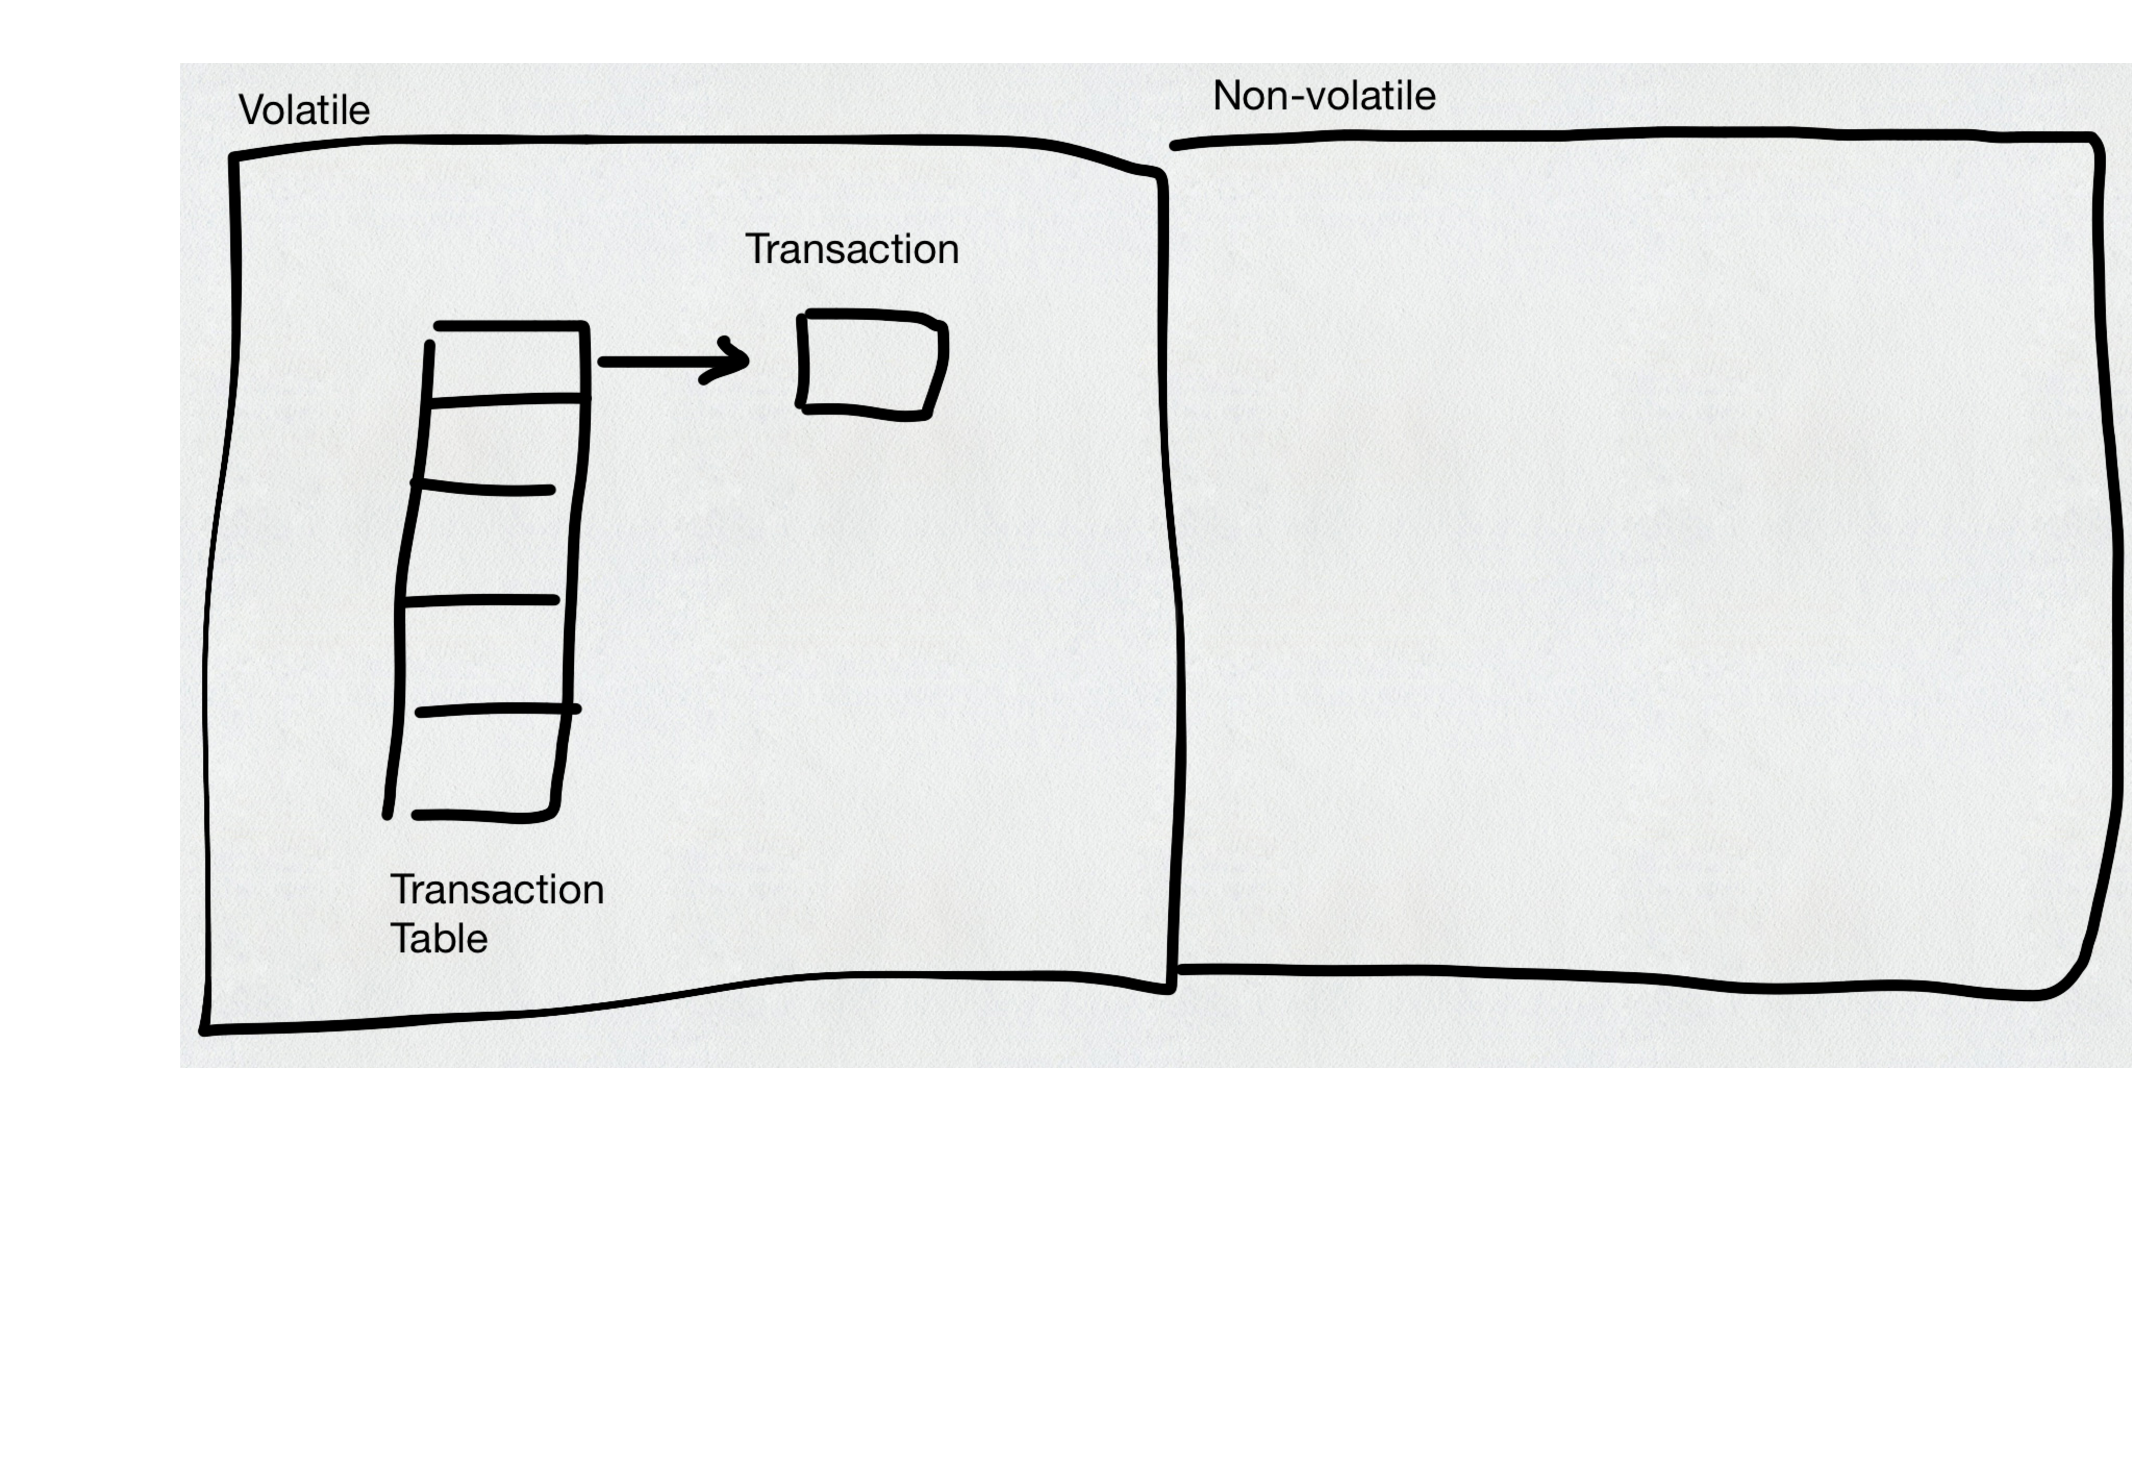
\includegraphics[width=\textwidth]{figures/drafts/concept-struct-volatile.pdf}
    \caption{}
    \label{fig:concept-struct-volatile}
\end{figure}

\subsubsection{Non-Volatile Section}

The non-volatile section stores all data that are durable across restarts. It
holds a control block, the index structure, and all data items mapped by the
index.

\paragraph{Control Block}

The control block is used to store a few essential metadata and for locating the
index after a restart. For that purpose, the control block is placed in a fixed
position of the \ac{KVS}' non-volatile region. Possible locations are the front
or rear end of the memory region. The index can be found by storing an offset or
pointer. Either way, the underlying system must provide a way to reuse or
recover a previous memory mapping, so both location methods are sufficient.

\paragraph{Index}

The index implements the actual \ac{KVS} paradigm by mapping keys to individual
data items. Note that, due to \ac{MVCC}, instead of mapping concrete data items,
each key maps to a history of versions of its associated item. It is the core
data structure of a \ac{KVS} and accessed by all transactions concurrently. As
such, the index is a strong contention point that is also very critical for the
performance of the \ac{KVS}. For that reason, selecting a suitable data
structure is crucial. The domain analysis in Chapter \ref{ch:kvs-nvram} shows
that many, if not most, \acp{KVS} rely on hash tables. Reasons are amortized
constant access, well-known array-like allocation schemes, and comparably low
complexity. B-trees or radix trees, on the other hand, are slower and optimized
for disk storage which was shown to be inappropriate for \ac{NVRAM}. Therefore,
this work opts for an index based on a hash table.

Operations on the index include adding, retrieving, and removing a key-value
pair. To prevent inconsistencies through race conditions, access must be
mutually exclusive. While locking can quickly become a bottleneck in
read-dominated scenarios, non-blocking data structures are generally slower and
more complex. The actual hashing method is an implementation detail (see Chapter \ref{ch:impl}).

\paragraph{Histories}

The index maps each key to a chain of versions of a data item. Before an
operation on an item can begin, the \ac{MVCC} algorithm has to determine which
version of the item is visible to the requesting transaction. As a result,
histories may be iterated frequently. Also, multiple transactions may access the
same history at a time, so there may be overlapping accesses. However,
transactions never remove and only append new versions to the history.
Therefore, contention may be high but mostly read-only. In order to account for
these characteristics, an array-like data structure may be the most appropriate
choice as opposed to a list. Consecutive access in arrays is less likely to
cause page faults and can benefit from hardware prefetching. Also, arrays have
simpler allocation patterns compared to lists. Problems arise with garbage
collection which could perform random-access modifications to the history. Since
garbage collection would break the scope of this work, it is assumed to be
absent or as non-invasive as possible. The concrete data structure used for
histories is left to the implementation (see Chapter \ref{ch:impl}).

\todo[inline]{arrays are not so optimal for histories (lists are better for concurrency)}

\begin{figure}[h!]
    \centering
    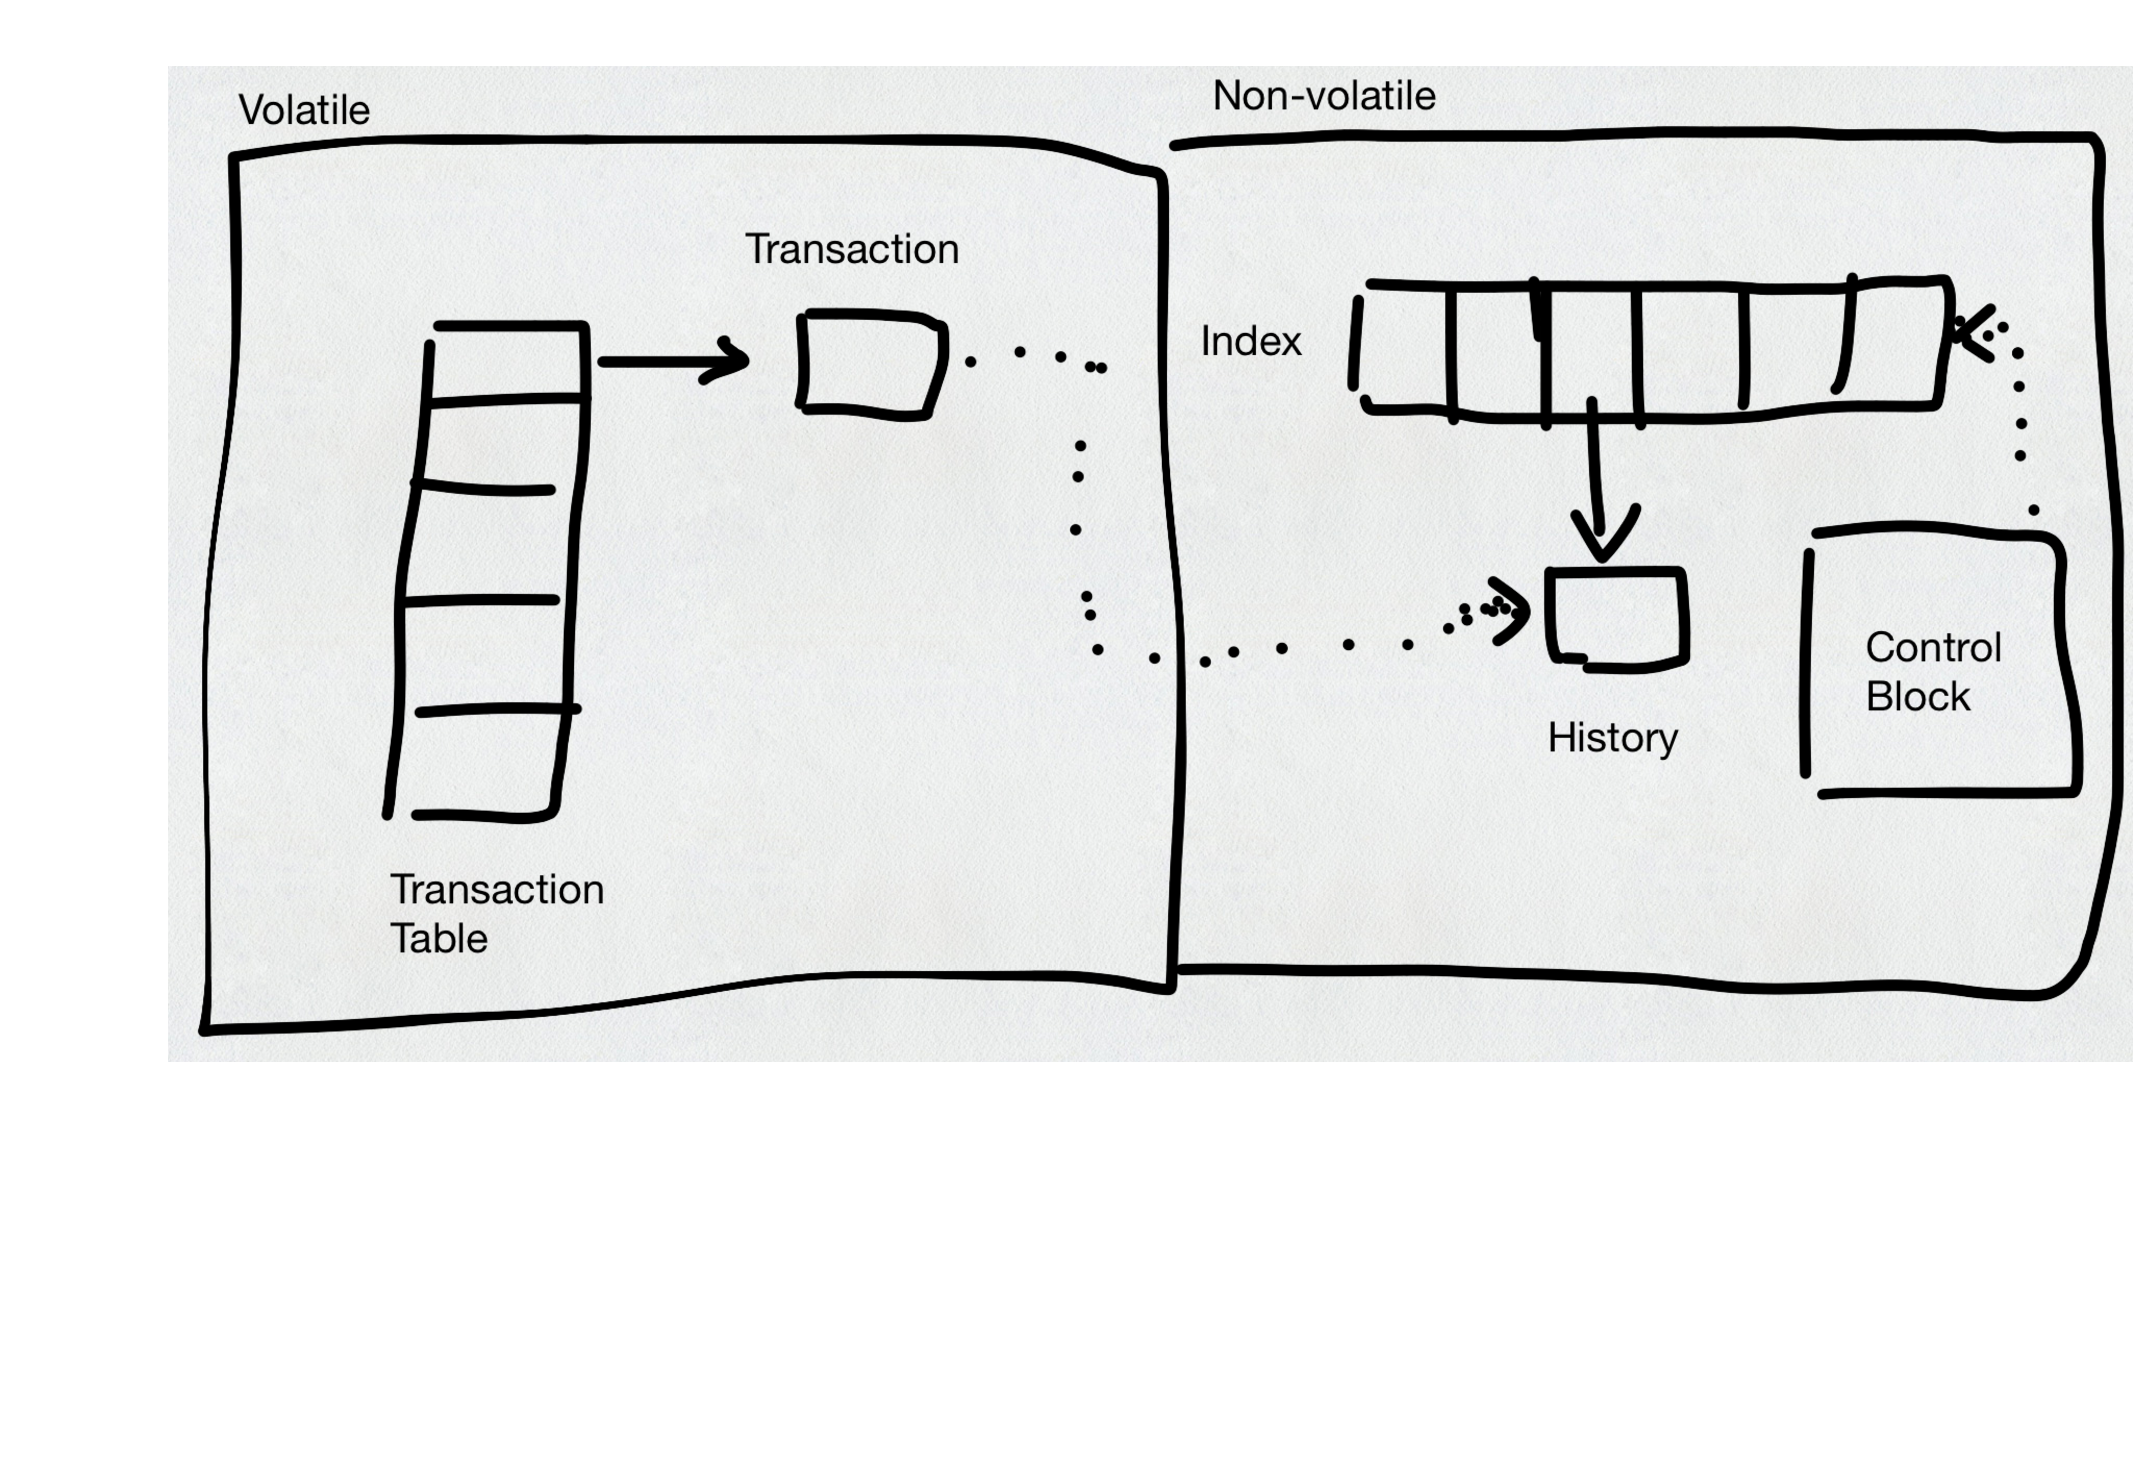
\includegraphics[width=\textwidth]{figures/drafts/concept-struct-complete.pdf}
    \caption{}
    \label{fig:concept-struct-complete}
\end{figure}


\section{Crash Consistency}
\label{ch:concept-consistency}
Posting updates to NVRAM is different from traditional non-volatile storage
media. With NVRAM, write-back is not directly observable by software and the
underlying memory subsystem is unaware of transactional semantics. As a result,
updates may be reordered or get stuck in store buffers and caches, thus
threatening consistency across crashes.

As pointed out in Chapter \ref{ch:nvram-consistency}, programmers need to
manually enforce write-back, in order to preserve consistency. At first, it is
important to enforce strict program order for transactionally related memory
operations. This can be done with memory barriers or fences. While such measures
usually include flushing store buffers, in-flight updates may still get stuck in
caches. To prevent this, cache line flushes or non-temporal stores could be
used. Even when reaching a memory controller, stores are once again buffered to
speed up subsequent reads to that item. While earlier works anticipated
designated flush instructions for controller buffers, both researchers and
hardware vendors have agreed on the platform feature ADR. When power fails, it
receives a signal and utilizes the remaining electrical energy to flush all
memory controller buffers.

With the exception of ADR, all of these methods can significantly increase
execution latencies as they work against many aspects of modern microprocessors.
Deferred write-backs for example are useful to decrease access times for
recently written data. Flushing store buffers, however, also affects data that
are not involved in transactions. In addition, enforcing strict program order
usually results in pipeline stalls. Since there are no other options at the
moment, programmers have to meticulously manage and optimize updates to NVRAM.

Summing up, preserving consistency across crashes is necessary but also
introduces adverse effects on performance. In accordance with recent research,
this work requires the following features

\begin{itemize}
    \item means to enforce program order for memory accesses
    % \item means to flush potential memory order buffers
    \item means to flush cashes or individual cache lines
    \item ADR
\end{itemize}

Both memory order enforcement and fine-grained cache flushes are provided by
many instruction sets including \code{x86\_64}, SPARC, and IBM POWER and zSeries
\cite{mckenney2007memory}. ADR, on the other hand, is a new platform feature
that is already supported on some systems. Therefore, no changes to existing
hardware are needed.


% \todo[inline]{Insert concluding example: e.g. structure w/ numbered arrows}
